% !TEX root = ../c3.tex

\section{Results}
\label{c3:sec:results}
From the joint model fitted to the PRIAS dataset, we found that both $\log_2 \{\mbox{PSA} + 1\}$ velocity, and log odds of having $\mbox{DRE} > \mbox{T1c}$ were significantly associated with the hazard of cancer progression. For any patient, an increase in $\log_2 \{\mbox{PSA} + 1\}$ velocity from -0.03 to 0.16 (first and third quartiles of the fitted velocities, respectively) corresponds to a 1.94 fold increase in the hazard of cancer progression. Whereas, an increase in odds of $\mbox{DRE} > \mbox{T1c}$ from -6.650 to -4.356 (first and third quartiles of the fitted log-odds, respectively) corresponds to a 1.40 fold increase in the hazard of cancer progression. Detailed results pertaining to the fitted joint model are presented in Appendix~\ref{c3:appendix_subsec:A_paramestimates}.

\subsection{Comparison of Various Approaches for Biopsies}
From the simulation study, we obtain the number of biopsies and the delay in detection of cancer progression for each of the ${\mbox{500} \times \mbox{250}}$ test patients using different schedules. Figure~\ref{c3:fig:5} shows that the personalized and PRIAS approaches fall in the region of a better balance between the median number of biopsies and the median delay than fixed/heuristic schedules. Next evaluate these schedules on the basis of both median and interquartile range (IQR) of the number of biopsies and delay (see Figure~\ref{c3:fig:6}). For brevity, only the most widely used annual and PRIAS schedules, the proposed personalized approach with fixed risk thresholds of 5\% and 10\%, and visit-specific threshold chosen using $\mbox{F}_1$ score are discussed next (see~Table~\ref{c3:table:app3} for remaining).

\begin{figure}
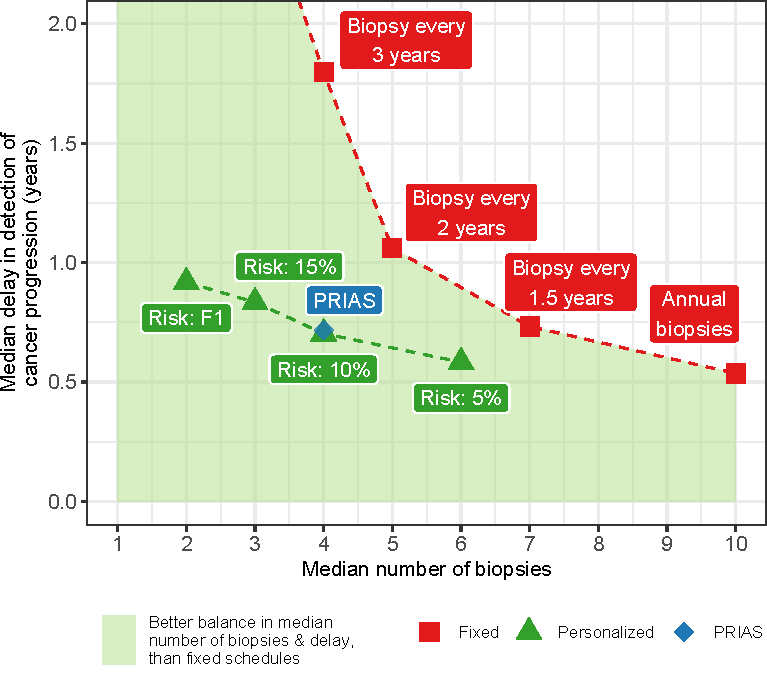
\includegraphics{contents/c3/images/c3_fig5.pdf}
\caption{\textbf{Burden-biopsy frontier:} Median number of biopsies (X-axis), and median delay in detection of cancer progression, in years (Y-axis), estimated from the simulation study. \textbf{Personalized schedules:} Risk:~15\%, Risk:~10\%, and Risk:~5\% approaches, schedule a biopsy if the cumulative-risk of cancer progression at a visit is more than 15\%, 10\%, and 5\%, respectively. Risk:~F1 works similarly, except that it utilizes a visit-specific threshold (see Section~\ref{c3:subsec:pers_decision_making}). The green shaded region depicts the region of better balance in the median number of biopsies and median delay than the currently practiced fixed/heuristic schedules.}
\label{c3:fig:5}
\end{figure}

Since patients have varying cancer progression speeds, the impact of each schedule also varies with it. To highlight these differences, we divide results for three types of patients, as per their time of cancer progression. They are \emph{fast, intermediate,} and \emph{slow progressing} patients. Although such a division may be imperfect and can only be done retrospectively in a simulation setting, we show results for these three groups for illustration. Roughly 50\% of the patients did not obtain cancer progression in the ten year follow-up period of the simulation study. We assume these patients to be \emph{slow progressing} patients. We assume \emph{fast progressing} patients are the ones with an initially misdiagnosed state of cancer~\citep{cooperberg2011outcomes} or high-risk patients who choose AS instead of immediate treatment upon diagnosis. These are roughly 30\% of the population, having a cancer progression time less than 3.5 years. We label the remaining 20\% patients as \emph{intermediate progressing} patients. 

\begin{figure}
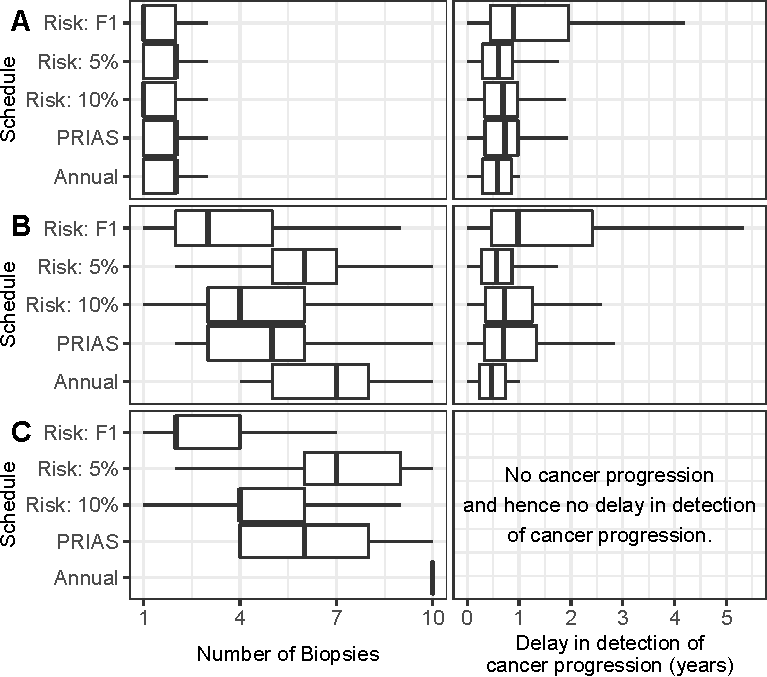
\includegraphics{contents/c3/images/c3_fig6.pdf}
\caption{Variation in the number of biopsies, and the delay in detection of cancer progression, in years, for various biopsy schedules. \textbf{Panel~A:} simulated patients with cancer progression times between 0 and 3.5 years (\emph{fast progressing}). \textbf{Panel~B:} simulated patients with progression times between 3.5 and 10 years (\emph{intermediate progressing}). \textbf{Panel~C:} simulated patients who did not have cancer progression in the ten years of follow-up (\emph{slow progressing}). \textbf{Personalized schedules:} Risk:~10\% approach schedules a biopsy at a visit if the corresponding cumulative-risk of cancer progression is more than 10\%. Risk:~5\% and Risk:~F1 work similarly, except that a visit-specific threshold is used in the latter (see Section~\ref{c3:subsec:pers_decision_making}). \textbf{Annual:} Yearly biopsies, and \textbf{PRIAS:} biopsies as per PRIAS protocol (see Section~\ref{c3:sec:introduction}).}
\label{c3:fig:6}
\end{figure}

For \emph{fast progressing} patients (Panel~A,~Figure~\ref{c3:fig:6}), we note that the personalized schedules with a fixed 10\% risk threshold and visit-specific threshold chosen using $\mbox{F}_1$ score, reduce one biopsy for 50\% of the patients, compared to PRIAS and annual schedule. Despite this, the delay (years) is similar for the personalized schedule with fixed 10\% risk threshold (median:~0.7,~IQR:~0.3--1.0), and the commonly used annual (median:~0.6,~IQR:~0.3--0.9) and PRIAS (median:~0.7,~IQR:~0.3--1.0) schedules.

For \emph{intermediate progressing} patients (Panel~A,~Figure~\ref{c3:fig:6}), we note that the delay (years) due to personalized schedule with fixed 5\% risk threshold (median:~0.6,~IQR:~0.3--0.9) is comparable to that of annual schedule (median 0.5,~IQR:~0.2--0.7). However, it schedules fewer biopsies (median:~6,~IQR:~5--7) than the annual schedule (median:~7,~IQR:~5--8). The delay (years) for PRIAS (median:~0.7,~IQR:~0.3--1.3) and personalized schedule with fixed 10\% risk (median:~0.7,~IQR:~0.4--1.3) are similar, but the personalized approach schedules one less biopsy for 50\% of the patients. Although the approach with the visit-specific risk threshold chosen using $\mbox{F}_1$ score schedules fewer biopsies than the 10\% fixed risk approach, it also has a higher delay.

The patients who are at the most advantage with the personalized schedules are the \emph{slow progressing} patients. These are a total of 50\% patients who did not progress during the entire study. Hence, the delay is not available for these patients (Panel~C of Figure~\ref{c3:fig:6}). For all of these patients, the annual schedule leads to 10 (unnecessary) biopsies. The schedule of the PRIAS program schedules a median of six biopsies (IQR:~4--8). In comparison, the biopsies scheduled by the personalized schedules using fixed 10\% risk threshold (median:~4,~IQR:~4--6) and visit-specific risk chosen using $\mbox{F}_1$ score (median:~2,~IQR:~2--4), are much fewer.

Overall, we observed that the personalized schedule which uses a 10\% risk threshold at all follow-up visits is dominant over the PRIAS schedule, biennial schedule of biopsies, and biopsies every one and a half years (see~Table~\ref{c3:table:app3} for the latter two schedules). This personalized schedule not only schedules fewer biopsies than the aforementioned currently practiced schedules, but the delay in the detection of cancer progression is also either equal or less. The personalized schedule, which uses the risk threshold chosen based on classification accuracy ($\mbox{F}_1$ score) is dominant over the triennial schedule of biopsies. The personalized schedule which uses a 5\% risk threshold schedules fewer biopsies than the annual schedule, while the delay is only trivially more than the annual schedule.